%&"../ai"
\endofdump
\tikzexternalize[prefix=cache/]{project1}
\begin{document}
    \title{项目一:MSA}
    \maketitle
    % 1)对算法的描述以及算法实现结果分析;
    % 2)不同算法的搜索结果;
    % 3)不同算法的运行时间;
    % 4)复杂度分析。

    \tableofcontents
    \clearpage

    \section{题目}

    \subsection{Topic}

    Implement three algorithms to solve multiple sequence alignment (MSA) problems.

    \subsection{Requirements}

    \begin{enumerate}
        \item Implement dynamic programming (DP) algorithm to find the optimal solution.
        \item Implement A-star (A$^\ast$) algorithm to find the optimal solution.
        \item Implement genetic algorithm to find the optimal/suboptimal solution.
    \end{enumerate}

    \subsection{Rules}

    \begin{table}[H]
        \centering
        \caption{Cost Matrix}\label{tab:costmat}
        \begin{tabular}{cccc}
            \toprule
                & Match $\alpha(p,p)$ & Mismatch $\alpha(p,q)$ & Gap $\delta$ \\
            \midrule
            Cost & 0 & 3 & 2 \\
            \bottomrule
        \end{tabular}
    \end{table}

    The table above shows the pairwise cost matrix. For multiple sequence alignment, the cost should be calculated in a cycle pairwise manner. Note that GAP-GAP is a match and should be considered as 0 cost. For every query, find the best alignment(s) in the database with the lowest cost.

    \section{动态规划算法}

    \subsection{双序列比对}

    在算法与复杂性课程\cite{algcom}里,已经提到了双序列比对的动态规划算法,如图 \ref{fig:pairwisedp} 所示,双序列比对对于一个状态只需要考虑三个临近状态的转移,分别是对齐$\alpha$,间隔 $\delta_x$、$\delta_y$,转换行动如表 \ref{tab:pairwise} 所示。对于每一个状态,都需要考虑经过哪一条路径消耗最小,于是就有了如算法 \ref{alg:pairwise} 的动态规划状态转移方程。

    \begin{algorithm}[H]
        \caption{双序列比对动态规划 MSA}\label{alg:pairwise}
        \KwIn{$x_1x_2\cdots x_m, y_1y_2\cdots y_n,\alpha,\delta$}
        \KwOut{minimum cost}
        \BlankLine
        \lFor{$i\leftarrow 0$ to $m$}{$M[i,0]=i\delta$}
        \lFor{$j\leftarrow 0$ to $n$}{$M[0,j]=j\delta$}
        \For{$i\leftarrow 1$ to $m$}{
            \For{$j\leftarrow 1$ to $n$}{
                $M[i,j]=\min(\alpha[x_i,y_j] + M[i-1,j-1], \delta + M[i-1,j], \delta + M[i,j-1])$\;
            }
        }
        \Return{$M[m,n]$}\;
    \end{algorithm}

    \begin{minipage}{0.48\textwidth}
        \begin{table}[H]
            \centering
            \caption{双序列行动坐标变换表}\label{tab:pairwise}
            \begin{tabular}{crr}
                \toprule
                    & $i$ & $j$ \\
                \midrule
                $\alpha$ & $+1$ & $+1$ \\
                $\delta_x$ & $0$ & $+1$ \\
                $\delta_y$ & $+1$ & $0$ \\
                \bottomrule
            \end{tabular}
        \end{table}
    \end{minipage}\hfil
    \begin{minipage}{0.48\textwidth}
        \begin{figure}[H]
            \centering
            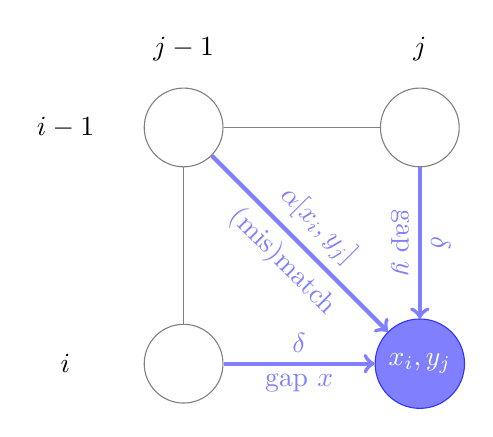
\begin{tikzpicture}
\tikzstyle{strnode}=[circle,draw=gray,minimum width=1cm];
\tikzstyle{move}=[line width=1.5pt, blue!50, ->];
\node[strnode] (v1) at (-1,0.5) {};
\node [strnode] (v3) at (2,0.5) {};
\node [strnode] (v4) at (-1,-2.5) {};
\node [strnode,fill=blue!50,draw=blue!80,font=\color{white}\bfseries] (v2) at (2,-2.5) {$x_i,y_j$};
\draw [move] (v1) edge node[sloped,above] {$\alpha[x_i,y_j]$} node[sloped,below] {(mis)match} (v2);
\draw [move] (v3) edge node[sloped,above] {$\delta$} node[sloped,below] {gap $y$} (v2);
\draw [move] (v4) edge node[sloped,above] {$\delta$} node[sloped,below] {gap $x$} (v2);
\draw[gray] (v1) edge (v3);
\draw[gray] (v1) edge (v4);
\node at (-2.5,0.5) {$i-1$};
\node at (-2.5,-2.5) {$i$};
\node at (2,1.5) {$j$};
\node at (-1,1.5) {$j-1$};
\end{tikzpicture}
            \caption{动态规划双序列比对}\label{fig:pairwisedp}
        \end{figure}
    \end{minipage}
    \medskip
    
    \subsection{多序列比对}\label{sec:mdp}

    对于三序列比对,情况就复杂地多,需要同时考虑七条路径。

    \begin{minipage}{0.48\textwidth}
        \begin{table}[H]
            \centering
            \caption{三序列行动坐标变换表}\label{tab:multiple}
            \begin{tabular}{crrr}
                \toprule
                    & $k$ & $j$ & $i$ \\
                \midrule
                $\alpha_x\delta_y\delta_z$  & 0 & 0 & 1\\
                $\delta_x\alpha_y\delta_z$ & 0 & 1 & 0 \\
                $\delta_x\alpha_y\alpha_z$ & 0 & 1 & 1 \\
                $\delta_x\delta_y\alpha_z$ & 1 & 0 & 0 \\
                $\alpha_x\delta_y\alpha_z$ & 1 & 0 & 1 \\
                $\alpha_x\alpha_y\delta_z$ & 1 & 1 & 0 \\
                $\alpha_x\alpha_y\alpha_z$ & 1 & 1 & 1 \\
                \bottomrule
            \end{tabular}
        \end{table}
    \end{minipage}\hfil
    \begin{minipage}{0.48\textwidth}
        \begin{figure}[H]
            \centering
            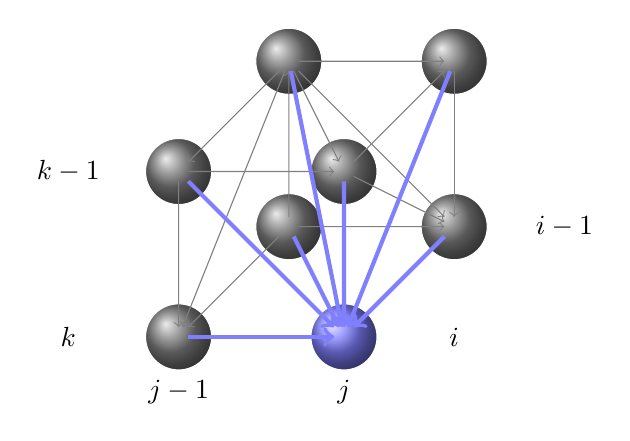
\begin{tikzpicture}[scale=1.4]
\tikzstyle{strnode}=[ball color=gray,white];
\tikzstyle{move}=[line width=1.5pt, blue!50, ->];
\tikzstyle{nomoce} = [gray, ->]
\draw[strnode] (-1.5,1.5) node (v1) {} circle (0.3cm);
\draw[strnode] (-1.5,3) node (v5) {} circle (0.3cm);
\draw[strnode] (0,3) node (v7) {} circle (0.3cm);
\draw[strnode] (0,1.5) node (v4) {} circle (0.3cm);
\draw[strnode, ball color=blue!50] (-1,0.5) node (v2) {} circle (0.3cm);
\draw[strnode] (-2.5,0.5) node (v3) {} circle (0.3cm);
\draw[strnode] (-2.5,2) node (v8) {} circle (0.3cm);
\draw[strnode] (-1,2) node (v6) {} circle (0.3cm);
\draw [nomoce] (v5) edge (v7);
\draw [nomoce] (v7) edge (v4);
\draw [nomoce] (v5) edge (v8);
\draw [nomoce] (v8) edge (v6);
\draw [nomoce] (v6) edge (v7);
\draw [nomoce] (v8) edge (v3);
\draw [nomoce] (v6) edge (v4);
\draw [nomoce] (v5) edge (v6);
\draw [nomoce] (v1) edge (v3);
\draw [nomoce] (v1) edge (v4);
\draw [nomoce] (v1) edge (v5);
\draw [nomoce] (v5) edge (v4);
\draw [nomoce] (v5) edge (v3);
\draw [move] (v1) edge (v2);
\draw [move] (v3) edge (v2);
\draw [move] (v4) edge (v2);
\draw [move] (v5) edge (v2);
\draw [move] (v6) edge (v2);
\draw [move] (v7) edge (v2);
\draw [move] (v8) edge (v2);
\node at (1,1.5) {$i-1$};
\node at (0,0.5) {$i$};
\node at (-1,0) {$j$};
\node at (-2.5,0) {$j-1$};
\node at (-3.5,0.5) {$k$};
\node at (-3.5,2) {$k-1$};
\end{tikzpicture}
            \caption{动态规划三序列比对}\label{fig:multipledp}
        \end{figure}
    \end{minipage}
    \medskip

    可以统一化为多序列比对问题。对于 $L$ 条序列比对,首先需要递归地初始化低维度边缘(如图 \ref{fig:downdim} 所示,注意附加高维度的间隙,高维度以间隙填充表示),之后余下空间其行动转换方法可以被表示为二进制从 $(\underbrace{0\cdots01}_{L\text{ digits}})_2$ 到 $(\underbrace{1\cdots11}_{L\text{ digits}})_2$ 内所有的数(最低位为第一维度),计算损耗使用上三角成对比较,规则统一为
    \begin{equation*}
        \texttt{compare}=
        \begin{cases}
            0,& (-,-) \| (p,p) \\
            2,& (p,-) \| (-,q) \\
            3,& (p,q)
        \end{cases}
    \end{equation*}
    并在确定每一次行动后记录路径,最后回溯路径到原点。

    \begin{figure}[H]
        \centering
        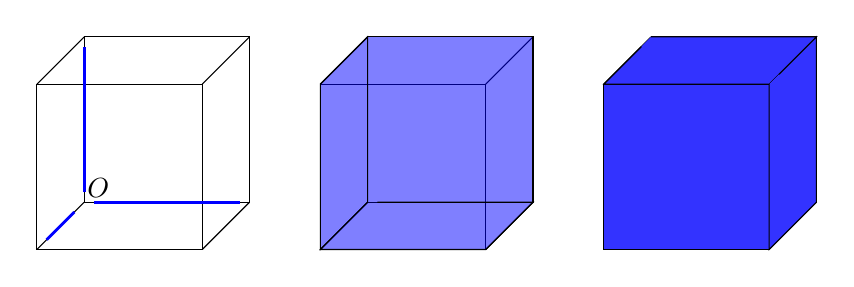
\begin{tikzpicture}[scale=0.6]
\tikzstyle{visited}=[line width=1pt,blue];

\draw  (-2.5,1.5) node (v2) {} rectangle (1,-2) node (v4) {};
\draw  (-1.5,2.5) node (v1) {} rectangle (2,-1) node (v3) {};
\draw (1,1.5) -- (2,2.5);
\draw (-1.5,-1) node (v7) {} -- (-2.5,-2) node (v9) {};
\draw (2,-1) node (v10) {} --  (1,-2);
\draw  (-1.5,2.5) node (v8) {} --  (-2.5,1.5) ;

\draw (7,1.5) -- (8,2.5);
\draw (4.5,-1) node (v11) {} -- (3.5,-2) node (v12) {};
\draw (8,-1) --  (7,-2);
\draw  (4.5,2.5) node (v6) {} --  (3.5,1.5) node (v5) {} ;
\draw  (v5) rectangle (7,-2) node (v15) {};
\draw [fill=blue,fill opacity=0.5] (v6) rectangle (8,-1) node (v16) {};
\draw [fill=blue,fill opacity=0.5] (4.5,2.5) --  (4.5,-1) node (v13) {} -- (3.5,-2) node (v14) {} -- (3.5,1.5) -- cycle;
\draw [fill=blue,fill opacity=0.5] (4.5,-1) -- (3.5,-2) -- (7,-2) -- (8,-1) -- (v13);

\draw (13,1.5) -- (14,2.5) node (v17) {};
\draw (10.5,-1) -- (9.5,-2);
\draw (14,-1) --  (13,-2);
\draw  (10.5,2.5) node (v6) {} --  (9.5,1.5) node (v5) {} ;
\draw  (v6) rectangle (14,-1) node (v20) {};
\draw [fill=blue!80]  (v5) rectangle (13,-2) node (v19) {};

\draw [visited] (v7) edge (v8);
\draw [visited] (v7) edge (v9);
\draw [visited] (v7) edge (v10);

\draw[fill=blue!80] (v6) -- (9.5,1.5) -- (13,1.5) node (v18) {} -- (14,2.5) node (v21) {} -- (10.5,2.5);

\draw[fill=blue!80] (13,1.5) -- (13,-2) --  (14,-1)  --(14,2.5)-- (v18);
\node at (-1.2,-0.7) {$O$};
\end{tikzpicture}
        \caption{降维递归}\label{fig:downdim}
    \end{figure}

    % 29s
    % > 24h
    % 8 核多线程进行中

    几乎类似于双序列比对,下面是 \verb"numpy" 实现版本,虽然其速度没有使用 Python 内置的 \verb"list" 版本(\href{./msa\_mdp.py}{\ttfamily msa\_mdp.py})的快,但是代码可读性已经与伪代码相当。

    \codeseg[language=python]{msa\_ndp.py}{9}{55}

    \subsection{运行时间}

    如果字符串平均长度为 $l$,该算法 $L$ 维字符串的复杂度为:
    \begin{equation}
        O_S = (2^L-1)\prod_{i=1}^L \texttt{len}(S[i]) = O(l^L)
    \end{equation}

    对于该问题,有 $m$ 个待比对序列,$n$ 个数据库项目,总时间复杂度为:
    \begin{equation*}
        mC_{n}^{L-1}O_S \approx mC_{n}^{L-1}l^L
    \end{equation*}

    实际运行时间如表 \ref{tab:dp},在服务器上运行时间如下。

    \begin{table}[h]
        \centering
        \caption{动态规划运行时间}\label{tab:dp}
        \begin{tabular}{cb{3cm}b{3cm}b{3cm}b{3cm}}
            \toprule
             &\multicolumn{2}{c}{\bfseries 双序列}  &\multicolumn{2}{c}{\bfseries 三序列} \\
             \cmidrule(r){2-3}\cmidrule(r){4-5} 
             & \bfseries 朴素实现 \href{./msa\_dp.py}{\ttfamily msa\_dp.py} &\bfseries \verb"list"实现 \href{./msa\_mdp.py}{\ttfamily msa\_mdp.py} &\bfseries \verb"list" 实现 \href{./msa\_mdp.py}{\ttfamily msa\_mdp.py} &\bfseries \verb"numpy" 实现 \href{./msa\_ndp.py}{\ttfamily msa\_ndp.py} \\
            \midrule
            运行时间 & 3s & 33s & 48h & $\sim$72h \\
            \bottomrule
        \end{tabular}
    \end{table}

    \section{A* 算法}

    \subsection{算法描述}

    A* 算法会从后继结点中首先扩展评估函数 $f(n)=g(n)+h(n)$ 最小的结点,如果 $h(n)$ 的选择满足可满足启发式和一致性的性质,就可以找到按照贪婪算法的思想找到最优解。

    这里将会非常乐观地估计剩下的字符串剩余部分都可以完美匹配,只会剩余间隔损耗。对于状态为 $n$ 的启发函数就可以被定义为轮换剩余长度差的和之下界
    \begin{equation*}
        \delta\sum_{cyc} \left|(l_1-\texttt{pos}[i])-(l_2-\texttt{pos}[j])\right| \geq \delta \left(L\max a_i - \sum_i a_i\right) = h(n)
    \end{equation*}
    其中
    \begin{equation*}
        a_i = l_i - \texttt{pos}[i]
    \end{equation*}

    % 这种由乐观得到的启发函数使得对角线上的每一步都被估计为 0,易证为满足\textbf{可满足启发式}。

    不等式容易从下面图 \ref{fig:gap} 的可视分析中论证,这样选择的 $h(n)$ 满足\textbf{可满足启发式}。

    \begin{figure}[H]
        \centering
        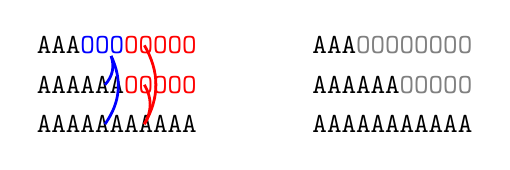
\begin{tikzpicture}[font=\ttfamily,line width=1pt]
\node[right] at (-2,1) {AAA\color{blue}OOO\color{red}OOOOO};
\node[right] at (-2,0.5) {AAAAAA\color{red}OOOOO};
\node[right] at (-2,0) {AAAAAAAAAAA};
\draw[bend left,blue] (-1,1) node (v1) {} edge (-1,0.5);
\draw[bend left,blue] (v1) edge (-1,0);
\draw[bend left,red] (-0.5,1) edge (-0.5,0) node (v2) {};
\draw[bend left,red] (-0.5,0.5) edge (-0.5,0);
\node[right] at (1.5,1) {AAA\color{gray}OOOOOOOO};
\node[right] at (1.5,0.5) {AAAAAA\color{gray}OOOOO};
\node[right] at (1.5,0) {AAAAAAAAAAA};
\end{tikzpicture}
        \caption{每一个间隔都至少贡献了一次}\label{fig:gap}
    \end{figure}

    之后来证明\textbf{一致性}。对于 A* 算法而言,其下一步的定义如图 \ref{fig:pairwiseastar} 和 \ref{fig:multipleastar} 所示。此处每一步的损耗都会大于等于0,而这种最好情况只会在全部序列都减少了 1 长度才会产生(超体对角线),这种情况下$h(n)=h(n^\prime)$;由于坐标至少在某一维度上增加了 1,一旦产生了间隙,就会有至少 2 的损耗,但是启发函数只会对应地减少 1,所以这个函数将满足一致性:
    \begin{equation*}
        h(n)\leq c(n,a,n^\prime) + h(n^\prime)
    \end{equation*}

    \begin{figure}[H]
        \centering
        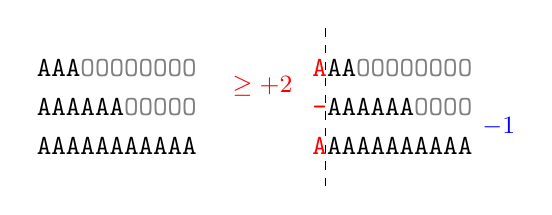
\begin{tikzpicture}[font=\ttfamily,line width=1pt]
\node[right] at (1.5,1) {AAA\color{gray}OOOOOOOO};
\node[right] at (1.5,0.5) {AAAAAA\color{gray}OOOOO};
\node[right] at (1.5,0) {AAAAAAAAAAA};
\node[right] at (5,1) {\color{red}A\color{black}AA\color{gray}OOOOOOOO};
\node[right] at (5,0.5) {\color{red}-\color{black}AAAAAA\color{gray}OOOO};
\node[right] at (5,0) {\color{red}A\color{black}AAAAAAAAAA};
\node[above] at (4.5,0.5) {\small \color{red} $\geq +2$};
\node[below] at (7.5,0.5) {\small \color{blue} $-1$};
\draw[dashed,line width=0.5pt] (5.3,1.5) -- (5.3,-0.5);
\end{tikzpicture}
        \caption{前进一步的不等式贡献}\label{fig:gaptri}
    \end{figure}

    \begin{figure}[h]
        \centering
        \begin{minipage}{0.48\textwidth}
            \centering
            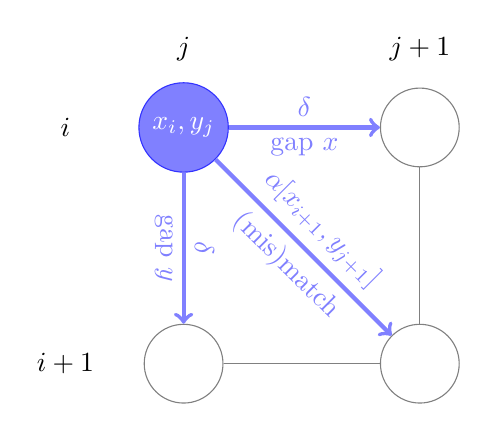
\begin{tikzpicture}
\tikzstyle{strnode}=[circle,draw=gray,minimum width=1cm];
\tikzstyle{move}=[line width=1.5pt, blue!50, ->];
\node[strnode,fill=blue!50,draw=blue!80,font=\color{white}\bfseries] (v1) at (-1,0.5) {$x_i,y_j$};
\node [strnode] (v3) at (2,0.5) {};
\node [strnode] (v4) at (-1,-2.5) {};
\node [strnode] (v2) at (2,-2.5) {};
\draw [move] (v1) edge node[sloped,above] {$\alpha[x_{i+1},y_{j+1}]$} node[sloped,below] {(mis)match} (v2);
\draw [gray] (v3) edge (v2);
\draw [gray] (v4) edge (v2);
\draw[move] (v1) edge node[sloped,above] {$\delta$} node[sloped,below] {gap $x$} (v3);
\draw[move] (v1) edge node[sloped,above] {$\delta$} node[sloped,below] {gap $y$} (v4);
\node at (-2.5,0.5) {$i$};
\node at (-2.5,-2.5) {$i+1$};
\node at (2,1.5) {$j+1$};
\node at (-1,1.5) {$j$};
\end{tikzpicture}
            \caption{A* 双序列比对}\label{fig:pairwiseastar}
        \end{minipage}
        \begin{minipage}{0.48\textwidth}
            \centering
            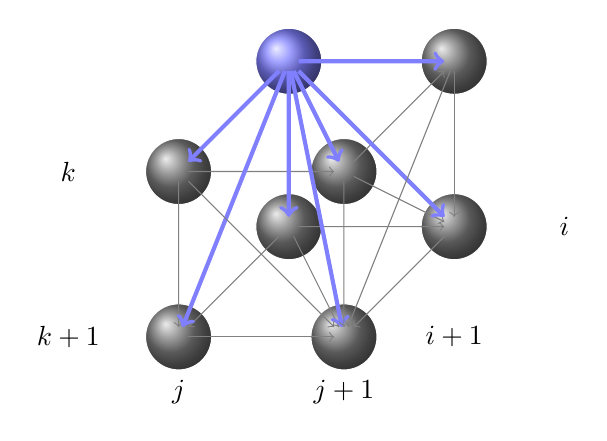
\begin{tikzpicture}[scale=1.4]
\tikzstyle{strnode}=[ball color=gray,white];
\tikzstyle{move}=[line width=1.5pt, blue!50, ->];
\tikzstyle{nomoce} = [gray, ->]
\draw[strnode] (-1.5,1.5) node (v1) {} circle (0.3cm);
\draw[strnode, ball color=blue!50] (-1.5,3) node (v5) {} circle (0.3cm);
\draw[strnode] (0,3) node (v7) {} circle (0.3cm);
\draw[strnode] (0,1.5) node (v4) {} circle (0.3cm);
\draw[strnode] (-1,0.5) node (v2) {} circle (0.3cm);
\draw[strnode] (-2.5,0.5) node (v3) {} circle (0.3cm);
\draw[strnode] (-2.5,2) node (v8) {} circle (0.3cm);
\draw[strnode] (-1,2) node (v6) {} circle (0.3cm);
\draw [move] (v5) edge (v7);
\draw [nomoce] (v7) edge (v4);
\draw [move] (v5) edge (v8);
\draw [nomoce] (v8) edge (v6);
\draw [nomoce] (v6) edge (v7);
\draw [nomoce] (v8) edge (v3);
\draw [nomoce] (v6) edge (v4);
\draw [move] (v5) edge (v6);
\draw [nomoce] (v1) edge (v3);
\draw [nomoce] (v1) edge (v4);
\draw [move] (v5) edge (v1);
\draw [move] (v5) edge (v4);
\draw [move] (v5) edge (v3);
\draw [nomoce] (v1) edge (v2);
\draw [nomoce] (v3) edge (v2);
\draw [nomoce] (v4) edge (v2);
\draw [move] (v5) edge (v2);
\draw [nomoce] (v6) edge (v2);
\draw [nomoce] (v7) edge (v2);
\draw [nomoce] (v8) edge (v2);
\node at (1,1.5) {$i$};
\node at (0,0.5) {$i+1$};
\node at (-1,0) {$j+1$};
\node at (-2.5,0) {$j$};
\node at (-3.5,0.5) {$k+1$};
\node at (-3.5,2) {$k$};
\end{tikzpicture}
            \caption{A* 三序列比对}\label{fig:multipleastar}
        \end{minipage}
    \end{figure}

    伪代码描述如算法 \ref{alg:astar} 所示\cite{astarwiki},其中可选行动随着坐标的不同可能会被限制,这样就会首先扩展评估函数最小的结点。

    \begin{algorithm}[h]
        \caption{A* 多序列比对}\label{alg:astar}
        \KwIn{$L$个字符串列表$S$,$\alpha$,$\delta$}
        \KwOut{minimum cost}
        \BlankLine
        $dist[\cdot]\leftarrow\infty$\;
        $move[\cdot]\leftarrow 0$\;
        $dist[start]\leftarrow 0$\;
        $move[start]\leftarrow 0$\;
        $openSet\leftarrow\textsc{Min-Heap}()$\;
        $openSet[start]=h(start)$\;
        $closeSet\leftarrow \{\}$\;
        \Repeat{$openSet$ is empty}{
            $current\leftarrow openSet$.pop()\;
            \If{$current$=$finish$}{
                \Return{$dist[current]$}\;
            }

            $closeSet$.add($current$)\;
            \ForEach{available move of $current$}{
                $n\leftarrow$\texttt{pos}$+$\emph{available move}\;
                $g(n)=dist(n)+\texttt{comparelist}(\textit{available move})$\;
                \If{$g(n)<dist[n]$}{
                    $move[n]\leftarrow$\emph{available move}\;
                    $dist[n]\leftarrow g(n)$\;
                    \If{$n$ not in $closeSet$}{
                        $openSet[n]\leftarrow g(n)+h(n)$\;
                    }
                }
            }
        }
        \Return{$\infty$}\;
    \end{algorithm}


    \subsection{运行时间}

    该算法的时间复杂度,对于 $L$ 个字符串(平均长度为 $l$),每一步的分支因子为 $2^{L}-1$,单个实例需要花费时间
    \begin{equation}
     < l^L \times (2^L-1) = O(l^L)
    \end{equation}
    因为这是一个树状结构的图,所以一定能够找到路径。扫描的节点数(第一项)要比动态规划小(如图 \ref{fig:path} 所示,由 \href{./compare.ipynb}{\ttfamily compare.ipynb} 生成),在常数级上会因为分支因子的多少而产生一定的差距。最多不会超过$\Theta((2^L-1)^{Ll})$(实际上应当多项式时间内即可,这个是 A* 的最差复杂度)。

    \begin{minipage}{0.5\textwidth}
        \begin{table}[H]
            \centering
            \caption{A* 运行时间}\label{tab:astar}
            \begin{tabular}{ccc}
                \toprule
                 & 双序列比对 & 三序列比对 \\
                \midrule
                运行时间 & 2min & 100h \\
                \bottomrule
            \end{tabular}
        \end{table}
    \end{minipage}
    \begin{minipage}{0.5\textwidth}
        \begin{figure}[H]
            \centering
            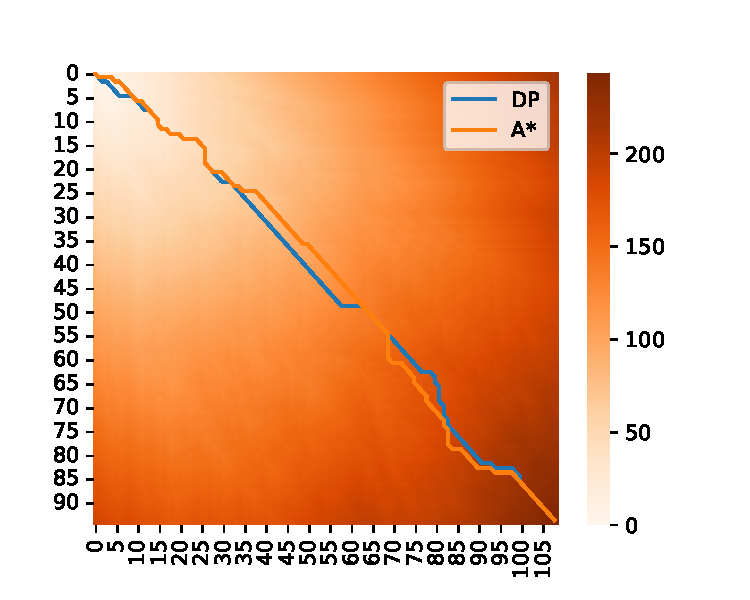
\includegraphics[width=\linewidth]{path}
            \caption{动态规划与A*扫描节点数上的比较}\label{fig:path}
        \end{figure}
    \end{minipage}

    \subsection{改进}

    但是从图 \ref{fig:path} 我们可以看到这个版本的 A* 仅筛除了 30\% 左右的节点,导致其运行速度依然很慢。需要选择一个更好的启发函数 $h(n)$ 以解决这个问题。

    该部分算法实现于\filelink{msa\_hastar.py}。启发函数可以使用轮换低维度反向损耗和以计算下界\cite{hastar}。根据表 \ref{tab:dp},二维动态规划是非常快的,尤其是使用专用加速的实现方法\filelink{msa\_dp.py},那么启发函数就可以定义为二维反向损耗轮换和
    \begin{equation*}
        h(n) = \sum_{i = 1}^L\sum_{j = i+1}^L R_{i,j}[\texttt{pos}[i],\texttt{pos}[j]]
    \end{equation*}
    式中 $R_{i,j}$ 为字符串反置$\overline{S_i}$和$\overline{S_j}$的距离矩阵$M_{\overline{i},\overline{j}}$(由二维动态规划算法 \ref{alg:pairwise} 定义)的对角反置,矩阵中每个点表示该位置距离匹配完成(右下角)的最小损耗,即
    \begin{equation*}
        R_{i,j} = [M_{\overline{i},\overline{j}}^T[0],M_{\overline{i},\overline{j}}^T[1],\cdots,M_{\overline{i},\overline{j}}^T[L]]^T
    \end{equation*}

    首先证明其\textbf{可满足性}。如图 \ref{fig:astarsat},如果在高维空间中剩余字符串的最短路径在低维度上的投影就是对应低维度上的低维最短路径,那么这个启发函数就是剩余距离(轮换定义的不同计算方法)。但大部分情况下,这种投影并不是对应的,在低维度上的投影很有可能会绕一些\emph{远路}而比纯粹的低维度最短路径要长。所以轮换低维度最小损耗和是真正剩余损耗的下界。
    \begin{equation*}
        h(n)\leq \texttt{cost} - g(n)
    \end{equation*}

    再证明其\textbf{一致性}。如图 \ref{fig:astarcon},采用\textbf{反证法},如果不满足一致性,则存在一个状态,其
    \begin{equation*}
        h(n)-h(n^\prime)> c(n,a,n^\prime)
    \end{equation*}
    意味着其低维最短路投影损耗之和超过了高维单步损耗。
    % 分为两种情况讨论:
    % \begin{enumerate}
    %     \item 如果高维单步投影到低维为一个间隙,这时不等式两边的贡献都是相等的 2,不会导致不等。
    %     \item 
    % \end{enumerate}
    事实上,考虑不等式两边的低维度分量(因为都是轮换定义的)
    \begin{equation*}
        \sum_k M_k(n) - \sum_k M_k(n^\prime) > \sum_k c_k(n,a,n^\prime)
    \end{equation*}
    即
    \begin{equation*}
        \sum_k\left(M_k(n)-M_k(n^\prime)-c_k(n,a,n^\prime)\right)>0
    \end{equation*}
    下面再用\textbf{反证法}证明$0\geq M_k(n)-M_k(n^\prime)-c_k(n,a,n^\prime)$。由于在计算低维度$M$矩阵时,如果 $c_k(n,a,n^\prime)<M_k(n)-M_k(n^\prime)$,对$M$来说,$n$是$n^\prime$的后继节点(反置所致),由于 $c_k(n,a,n^\prime)+M_k(n^\prime)<M_k(n)$,那么经过$n^\prime$是$n$的最短路径,应当有$c_k(n,a,n^\prime)+M_k(n^\prime)=M_k(n)$产生了矛盾。所以
    \begin{equation*}
        0\geq\sum_k\left(M_k(n)-M_k(n^\prime)-c_k(n,a,n^\prime)\right)
    \end{equation*}
    至此,两个式子产生了矛盾,所以$h(n)$符合一致性。

    \begin{figure}[H]
        \centering
        \begin{minipage}{0.48\textwidth}
            \centering
            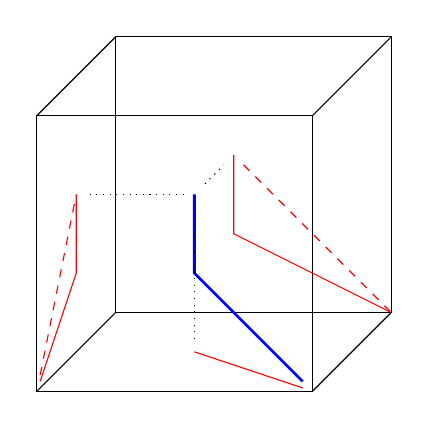
\begin{tikzpicture}
\tikzstyle{visited}=[line width=1pt,blue];

\draw  (-2.5,1.5) node (v2) {} rectangle (1,-2) node (v4) {};
\draw  (-1.5,2.5) node (v1) {} rectangle (2,-1) node (v3) {};
\draw (1,1.5) -- (2,2.5);
\draw (-1.5,-1) node (v7) {} -- (-2.5,-2) node (v9) {};
\draw (2,-1) node (v10) {} --  (1,-2) node (v5) {};
\draw  (-1.5,2.5) node (v8) {} --  (-2.5,1.5) ;


\draw[blue,line width=1pt] (-0.5,0.5) node (v12) {} -- (-0.5,-0.5) -- (0,-1) -- (v5);
\draw[red] (0,1) node (v6) {} -- (0,0) -- (2,-1);
\draw[red] (-0.5,-1.5) node (v13) {} -- (v5);
\draw[red] (-2,0.5) node (v11) {} -- (-2,-0.5) -- (v9);
\draw[red, dashed] (v6) -- (2,-1);
\draw[red, dashed] (v11) -- (v9);
\draw[dotted]  (v12) edge (v6);
\draw[dotted]  (v12) edge (v11);
\draw[dotted]  (v12) edge (v13);
\end{tikzpicture}
            \caption{改进后启发函数可满足性}\label{fig:astarsat}
        \end{minipage}
        \begin{minipage}{0.48\textwidth}
            \centering
            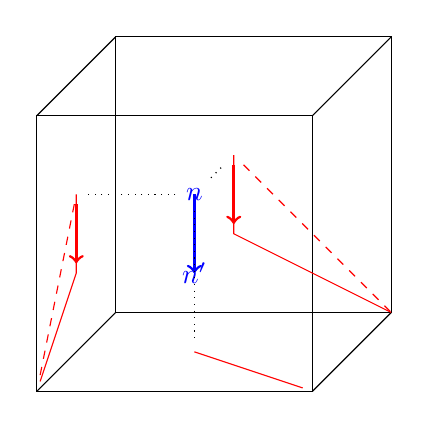
\begin{tikzpicture}
\tikzstyle{visited}=[line width=1pt,blue];

\draw  (-2.5,1.5) node (v2) {} rectangle (1,-2) node (v4) {};
\draw  (-1.5,2.5) node (v1) {} rectangle (2,-1) node (v3) {};
\draw (1,1.5) -- (2,2.5);
\draw (-1.5,-1) node (v7) {} -- (-2.5,-2) node (v9) {};
\draw (2,-1) node (v10) {} --  (1,-2) node (v5) {};
\draw  (-1.5,2.5) node (v8) {} --  (-2.5,1.5) ;


\draw[blue,line width=1pt,->] (-0.5,0.5) node (v12) {$n$} -- (-0.5,-0.5) node {$n^\prime$} ;
\draw[red] (0,1) node (v6) {} -- (0,0) node (v15) {} -- (2,-1);
\draw[red] (-0.5,-1.5) node (v13) {} -- (v5);
\draw[red] (-2,0.5) node (v11) {} -- (-2,-0.5) node (v14) {} -- (v9);
\draw[red, dashed] (v6) -- (2,-1);
\draw[red, dashed] (v11) -- (v9);
\draw[dotted]  (v12) edge (v6);
\draw[dotted]  (v12) edge (v11);
\draw[dotted]  (v12) edge (v13);
\draw[red, line width=1pt,->]  (v11) edge (v14);
\draw[red, line width=1pt,->]  (v6) edge (v15);
\end{tikzpicture}
            \caption{改进后启发函数一致性}\label{fig:astarcon}
        \end{minipage}
    \end{figure}

    大致算法如算法 \ref{alg:hastar} 所示。在时间复杂度上的分析,需要首先计算上述的矩阵,之后见图 \ref{fig:path2} 可以看到基本上筛除了 90\% 以上的节点,对于真正的 A* 部分而言几乎就是线性时间。

    \begin{equation}
        \underbrace{\sum_{i=1}^L\sum_{j=i+1}^L 3l_il_j}_{DP} + \underbrace{(2^L-1)\sum_{i=1}^L l_i}_{A^*} \approx 3C_{L}^2 l^2 + (2^L-1)Ll = O(l^2)
    \end{equation}

    \begin{algorithm}[h]
        \caption{改进后 A* 多序列比对}\label{alg:hastar}
        根据算法 \ref{alg:pairwise},计算每对反转字符串的距离矩阵$M$,并对角线反转得到 $R$\;
        设定启发函数$h(n)$为对应坐标轮换对应的$R$矩阵值的和\;
        按照算法 \ref{alg:astar},进行 A* 运算\;
    \end{algorithm}

    \begin{minipage}{0.5\textwidth}
        \begin{table}[H]
            \centering
            \caption{改进后 A* 运行时间}\label{tab:astar}
            \begin{tabular}{ccc}
                \toprule
                 & 双序列比对 & 三序列比对 \\
                \midrule
                运行时间 & 7s & 3h30min \\
                \bottomrule
            \end{tabular}
        \end{table}
    \end{minipage}
    \begin{minipage}{0.5\textwidth}
        \begin{figure}[H]
            \centering
            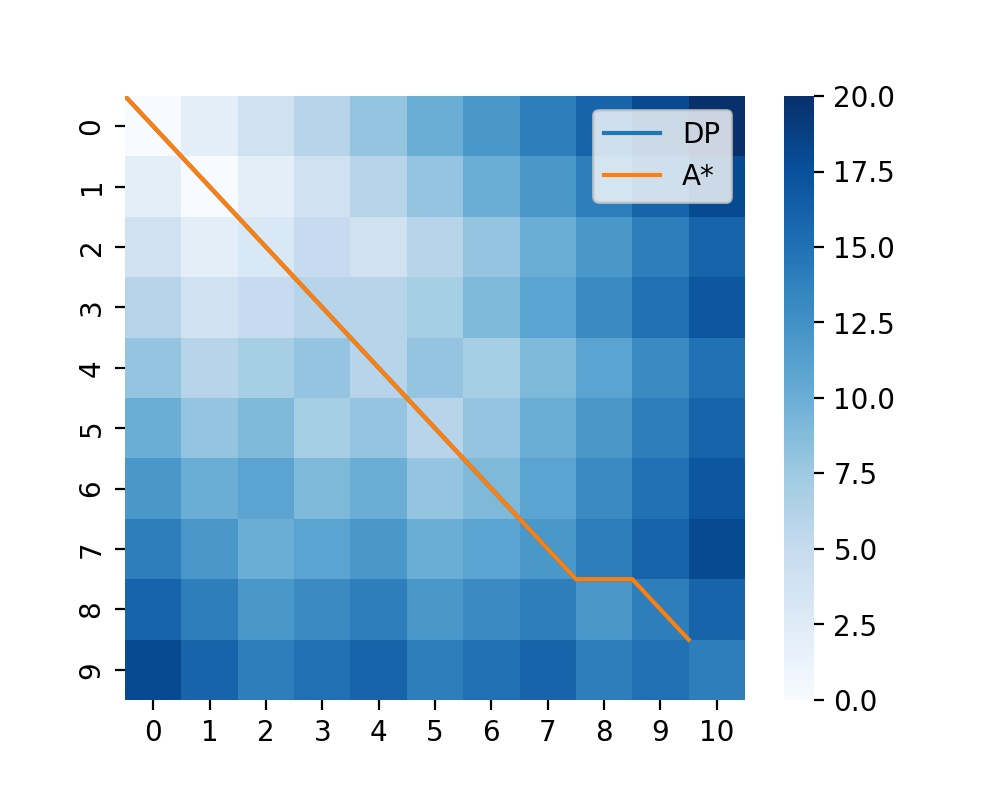
\includegraphics[width=\linewidth]{path2}
            \caption{动态规划与改进后A*扫描节点数比较}\label{fig:path2}
        \end{figure}
    \end{minipage}

    \section{遗传算法}

    \subsection{算法描述}
    
    % 简单遗传算法\cite{simplega} 在产生随机种群的时候使用了动态规划算法首先对每一对进行了预生成。

    \paragraph{初始化种群} 在构造随机状态的时候,首先需要考虑构造出的比对序列长度。经验\cite{simplega}告诉我们:
    \begin{equation*}
         l = k\max{(l_1,l_2,\cdots,l_n)}
    \end{equation*}
    中的缩放因子$k$取$(1.2,1.5)$区间内较为合适。然后分别向字符串插入对应数量的空格以对齐。不需要考虑同一位置全为空隙的情况,因为这样这个位置的损耗为 0。

    \paragraph{适应度函数} 将适应度函数定义为
    \begin{equation*}
        \mathit{fitness}(n) = l\alpha\frac{L(L-1)}{2} - cost(n)
    \end{equation*}
    表达与完全不匹配的距离。这个值越大,表明损耗越小,越有适应性。

    \paragraph{杂交算子} 均一化适应度函数后,按照对应概率选择亲本进行繁殖。繁殖的后代每一个字符串将会随机地选择其中一个亲本的对应性状。

    \paragraph{突变算子} 突变算子只能改变间隙,不能够修改字符(否则字符串比对就会不完整)。选中的子代随机选择一个字符串,移动其中一个间隙的位置。

    具体描述如算法 \ref{alg:ga} 所示。种群数目被设定为 1000,突变率被设置为 1 \%。

    \begin{algorithm}[H]
        \caption{遗传算法多序列比对}\label{alg:ga}
        \KwIn{$L$个字符串列表$S$,$\alpha$,$\delta$}
        \KwOut{minimum cost}
        \BlankLine
        $\mathit{population}\leftarrow$\texttt{initPopulation}($S$)\;
        \Repeat{max time is out}{
            $\mathit{new\_population}\leftarrow\varnothing$\;
            calculate $\mathit{pop\_fitness}$ for $\mathit{population}$\;
            \lIf{$\max{\textit{pop\_fitness}}>$threshold}{\textbf{break}}
            \For{$k\leftarrow 1$ to $\mathit{pop\_size}$}{
                $p_1,p_2\leftarrow$ choices from $\mathit{population}$ based on the $\mathit{pop\_fitness}$\;
                $\mathit{child}\leftarrow$\texttt{crossover}($p_1,p_2$)\;
                \lIf{mutation is triggered}{$\mathit{child}\leftarrow$\texttt{mutation}($\mathit{child}$)}
                $\mathit{new\_population}$.append($\mathit{child}$)\;
            }
            $\mathit{population}\leftarrow\mathit{new\_population}$\;
        }
        \Return{the best individual in $\mathit{population}$}\;
    \end{algorithm}

    \subsection{运行时间}

    运行时间主要取决于设定的时间阈值。对于双序列比对被设定为 5s,对于多序列比对被设定为 90s,并不一定得到最优解,因为繁衍可能不够完善,有可能得到次优解。

    \noindent
    \begin{minipage}{0.6\textwidth}
        \begin{table}[H]
            \centering
            \caption{遗传算法运行时间}\label{tab:ga}
            \begin{tabular}{ccc}
                \toprule
                 & 双序列比对 & 三序列比对 \\
                \midrule
                运行时间 & 45min & $\sim$ \\
                \bottomrule
            \end{tabular}
        \end{table}
    \end{minipage}
    \begin{minipage}{0.4\textwidth}
        \begin{figure}[H]
            \centering
            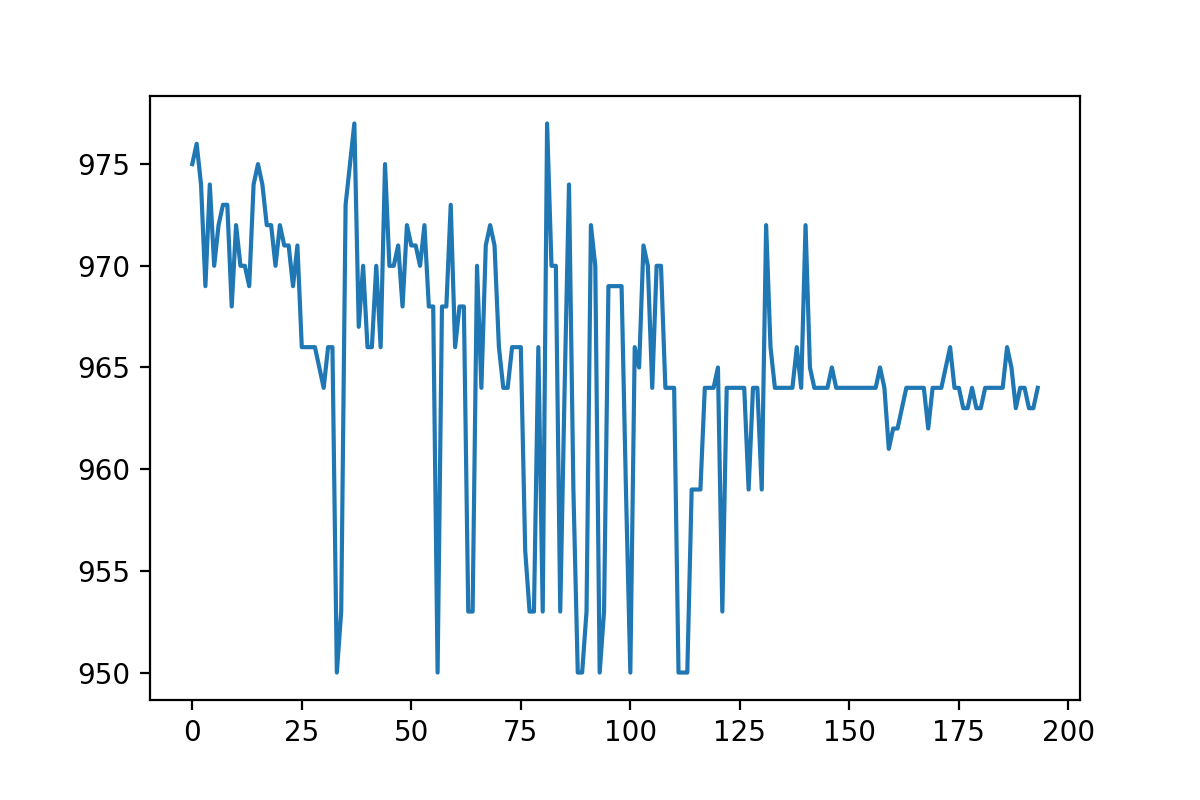
\includegraphics[width=\linewidth]{ga}
            \caption{遗传算法收敛情况}\label{fig:ga}
        \end{figure}
    \end{minipage}
    \vspace*{5pt}

    \subsection{改进}

    如图 \ref{fig:ga} 所示,现有的基本遗传算法收敛速度是相当慢的。为了让遗传算法的收敛速度更快,需要对初始化种群的方法进行改进。

    采用二维动态规划出的匹配序列进行初始化种群\cite{simplega},现在的字符串长度
    \begin{equation}
        l = k\max{(l_1,l_2,\cdots,l_n)}+x
    \end{equation}
    式子中 $x$ 为初始偏移最大值,取 $1.2\max_i{l_i}$,算法 \ref{alg:dpinit} 给出了初始化方法。

    \noindent
    \begin{minipage}{0.6\textwidth}
        \begin{algorithm}[H]
            \caption{基于动态规划的种群初始化}\label{alg:dpinit}
            对每一对字符串根据算法 \ref{alg:pairwise} 计算出最佳比对\;
            对于每一种群,每一个个体选择其中对应的一种匹配串,增加随机数量(不超过 $x$)的前缀间隔,后缀补齐间隔为预定字符串最大长度 $l$\;
        \end{algorithm}
    \end{minipage}
    \begin{minipage}{0.4\textwidth}
        \begin{figure}[H]
            \centering
            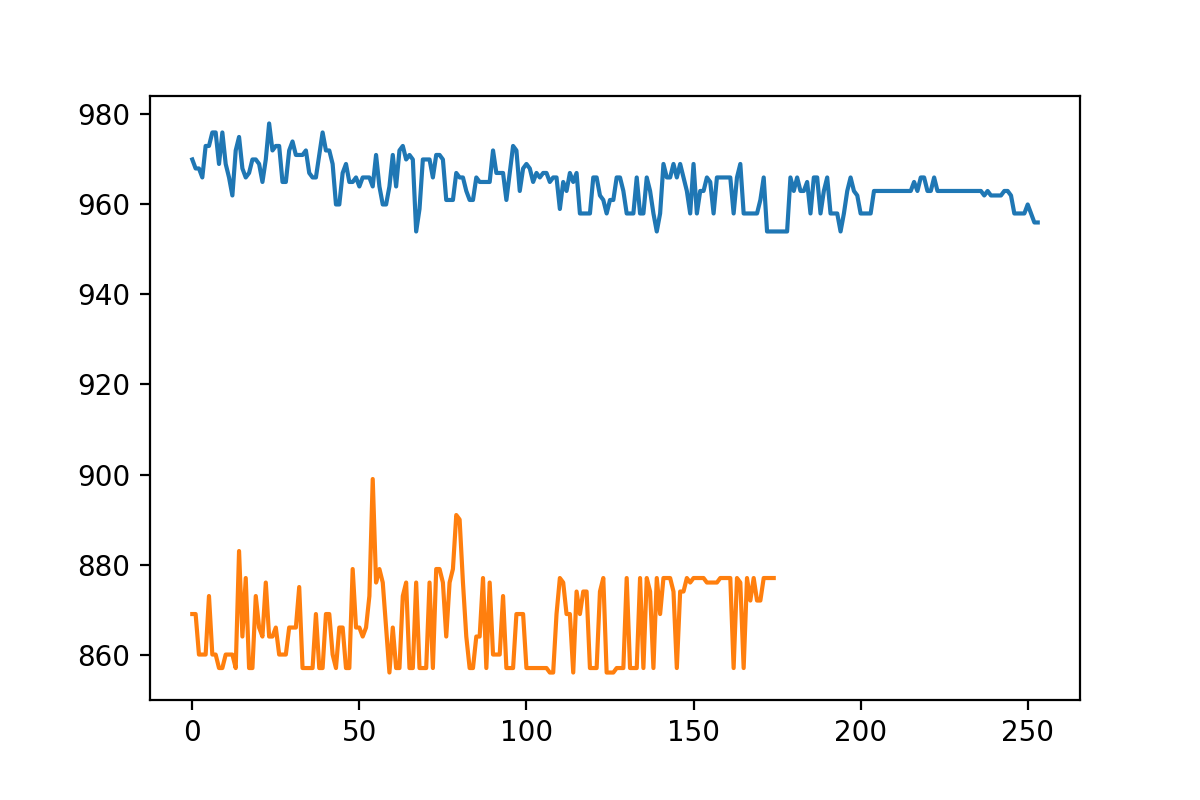
\includegraphics[width=\linewidth]{ga2}
            \caption{改进初始化种群后}\label{fig:ga2}
        \end{figure}
    \end{minipage}
    \vspace*{5pt}

    这种方法可以进行预对齐,图 \ref{fig:ga2} 可见其起点变得更低了。但是其减少速度却没有明显变化。这个时候需要修改适应度函数,基于\emph{内卷}的方法,将损耗最大的设置为最差的,并被\textbf{筛除},当前轮其余个体在损耗上与之的差值作为适应度函数。这样就是 1:1 对应的局部竞争,选择优秀个体繁衍后代,每一轮的标准都会有所不同。并且提高突变概率为 10\%,以提高多样性。图 \ref{fig:ga3} 显示了这种方法的更快的收敛速度。

    \noindent
    \begin{minipage}{0.6\textwidth}
        \begin{equation*}
            \mathit{fitness}(i) = \max_i(\texttt{cost}_i)-\texttt{cost}_i
        \end{equation*}
    \end{minipage}
    \begin{minipage}{0.4\textwidth}
        \begin{figure}[H]
            \centering
            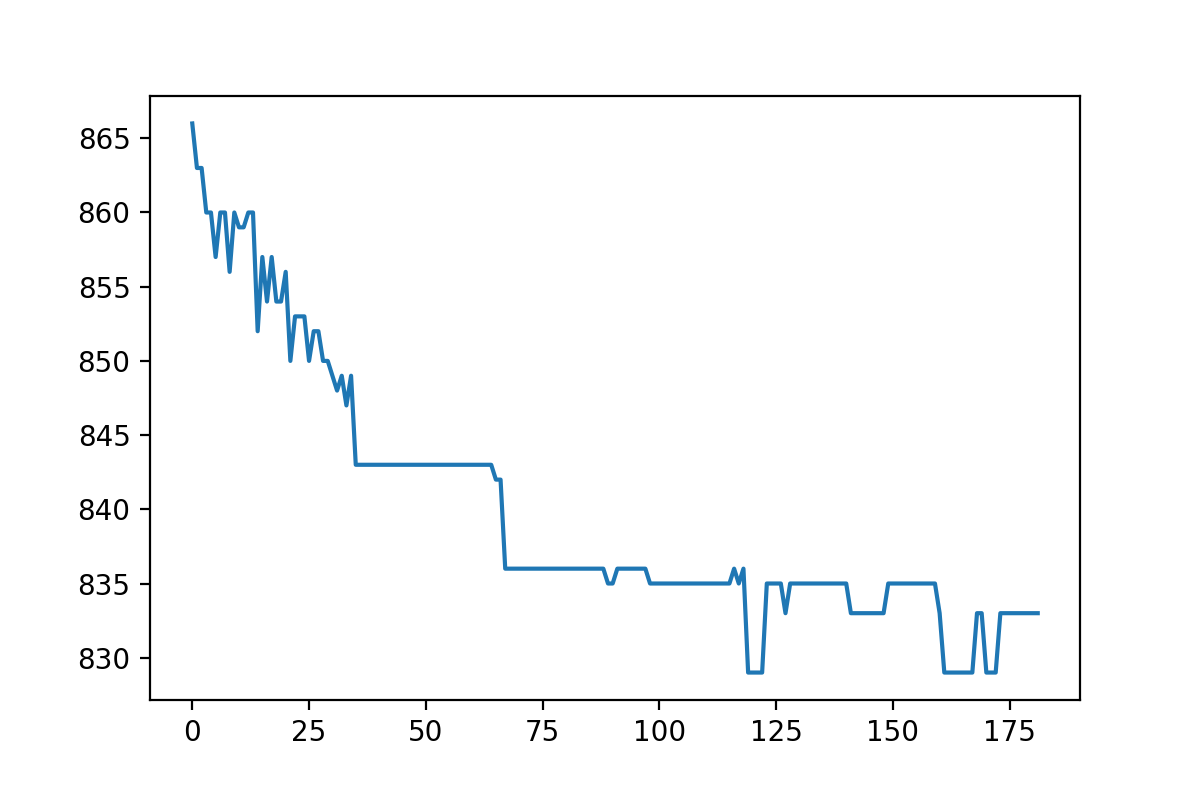
\includegraphics[width=\linewidth]{ga3}
            \caption{改进适应度函数后}\label{fig:ga3}
        \end{figure}
    \end{minipage}

    \section{运行}

    \subsection{运行框架}

    为了更好地进行代码复用,本工程采用如表 \ref{tab:framework} 的框架。

    \begin{table}[h]
        \caption{运行框架}\label{tab:framework}
    \begin{tabular}{|c|c|c|c|c|c|}
        \hline
        \multicolumn{6}{|c|}{\filelink{crosstest.py}(测试) \filelink{main.py}(计算)} \\
        \hline
        \filelink{msa\_dp.py} & \filelink{msa\_mdp.py} & \filelink{msa\_ndp.py} & \filelink{msa\_astar.py} & \filelink{msa\_hastar.py} & \filelink{msa\_ga.py}\\
        \hline
        \multicolumn{6}{|c|}{\filelink{msa\_util.py}}\\
        \hline        
    \end{tabular}
    \end{table}

    运行测试是为了使用一个样例进行交叉测试,以避免大型计算后才发现一些算法错误。直接运行主文件,会被询问用什么算法完成,并选择计算几维的样例。

    \subsection{运行结果}

    \bibliography{ref}

\end{document}